\documentclass[11pt]{amsart}
\usepackage{geometry}                % See geometry.pdf to learn the layout options. There are lots.
\geometry{letterpaper}                   % ... or a4paper or a5paper or ... 
%\geometry{landscape}                % Activate for for rotated page geometry
%\usepackage[parfill]{parskip}    % Activate to begin paragraphs with an empty line rather than an indent
\usepackage{graphicx}
\usepackage{amssymb}
\usepackage{epstopdf}
\DeclareGraphicsRule{.tif}{png}{.png}{`convert #1 `dirname #1`/`basename #1 .tif`.png}
\usepackage{amsfonts,amsmath,amsthm,amsbsy,latexsym,amssymb,graphicx,booktabs,multicol,color,fullpage}
\usepackage{mathabx,dashrule}
\usepackage{pgf,tikz}
\usepackage{pgfplots}
\usepackage{graphicx}
\usepackage{wrapfig}
\usepackage{multicol}
\usepackage{arydshln}
\usepackage{xcolor}



\title{A Numerically Stable Fourier Continuation Approximation for the Solution of Partial Differential Equations}
\author{Melanie Vining}
%\date{}                                           % Activate to display a given date or no date

\begin{document}
\maketitle
\section{Introduction} \\
\subsection{Motivation} \\
Our goal is to study a numerically accurate and stable scheme for solving partial differential equations on complex domains.  Several finite difference and finite element methods are available but have low-order accuracy.  We focus on the Fourier-Continuation Alternating-Direction (FC-AD)  method described by Bruno and Lyon in (citation needed!). This method gives a high-order unconditionally stable solver for partial differential equations on any smooth domain.  One of the interesting details in the FC-AD method is that the modification to the solution that yields unconditional stability is neither inherent to the problem nor an obvious choice and was in fact developed by numerical experiment.  We aim to find an unconditional stability condition that is more natural either to the problem itself or to the mechanics of the implementation (analyzing the singular values of the matrix, for example).  
\subsubsection{FC-AD}
The Fourier-Continuation Alternating-Direction algorithm is a method that applies the concept of Alternating Direction Implicit (ADI) methods to using a Fourier Continuation (FC) method in the spatial domain.  ADI methods reduce the numerical solution to PDEs into implicit first order boundary value problems in space.  In traditional ADI methods, these  BVPs are solved using finite-difference methods and yield low-accuracy results, particularly on the boundaries.  \\
Given the heat equation in two dimensions:
\begin{eqnarray}
u_t=k(u_xx+u_yy) + Q(x,y,t), & (x,y,t) \in \Omega \times (0,T], \nonumber \\
u(x,y,t) = G(x,y,t) & (x,y) \in \partial \Omega, t \in (0,T] \\
u(x,y,0)=u_0(x,y), & (x,y) \in \Omega, \nonumber 
\end{eqnarray}
with $k>0$, $\Omega \subset \mathbb{R}^2$ is smoothly bounded, and $Q$, $G$, and $u_0$ are smooth.  Discretizing according to $t^n=n\Delta t$, we then use a central difference scheme for the time derivative and enforce at $t^{n+\frac{1}{2}}=(n+\frac{1}{2})\Delta t$, resulting in
\begin{equation}
\dfrac{u^{n+1}-u^n}{\Delta t} = \dfrac{k}{2}\dfrac{\partial^2}{\partial x^2}(u^{n+1}-u^n) +\dfrac{k}{2}\dfrac{\partial^2}{\partial y^2}(u^{n+1}-u^n) + Q^{n+\frac{1}{2}} + E_1(x,y,\Delta t)
\end{equation}.
Here, $Q^{n+\frac{1}{2}}= Q(x,y,(n+\frac{1}{2})\Delta t)$ and $E_1(x,y,\Delta t)$ is the error term resulting from the central difference differentiation.  
Rearranging this equation gives us
\begin{equation}
(1-\dfrac{k\Delta t}{2}\dfrac{\partial ^2 }{\partial x ^2 } - \dfrac{k\Delta t}{2}\dfrac{\partial ^2 }{\partial y ^2 })u^{n+1}= (1+\dfrac{k\Delta t}{2}\dfrac{\partial ^2 }{\partial x ^2 } + \dfrac{k\Delta t}{2}\dfrac{\partial ^2 }{\partial y ^2 })u^n + Q^{n+\frac{1}{2}}+E_1(x,y,\Delta t)
\end{equation}
and then factoring the left hand side and moving extra terms over gives us
\begin{equation}
(1-\dfrac{k\Delta t}{2}\dfrac{\partial ^2}{\partial x^2} ) (1-\dfrac{k\Delta t}{2}\dfrac{\partial ^2}{\partial y^2} )u^{n+1} =  (1+\dfrac{k\Delta t}{2}\dfrac{\partial ^2}{\partial x^2} ) (1+\dfrac{k\Delta t}{2}\dfrac{\partial ^2}{\partial y^2} ) + \dfrac{k^2 \Delta t^2}{4}\dfrac{\partial ^ 2}{\partial x^2}\dfrac{\partial ^2}{\partial y ^ 2} (u^{n+1}-u^n) + \Delta t Q^{n + \frac{1}{2}} + \Delta t E_1(x,y,\Delta t)
\end{equation}



\subsubsection{FC Gram}
The FC Gram method matches points on a grid and applies a precomputed extension that results in a periodic function.  This resulting function can then be transformed via Fast Fourier Transform (FFT) in order to take derivatives. \\
We begin with a basis of functions, $f_0,f_1,\ldots,f_n$.  These functions can be any functions, but having an orthogonal basis or an orthonormal basis makes future computations much simpler.  Using the Gram Polynomials (also known as the Discrete Chebyshev Polynomials) is a natural option for this particular application of FC-Gram due to the equispaced points prescribed by the FC-AD Method.   These can be computed as point values using the desired grid via a QR factorization on a Vandermonde matrix.   
Then approximations with periodic extensions are then calculated for each function for a predetermined number of points $n$, giving us $f_{0_c},f_{1_c},\ldots f_{n_c}$.  Specifically, we choose to use the periodic extensions found when using the Fourier Continuation approximation method, hence the ``FC" in FC-Gram.  These approximations are stored as a basis.  

Next, we begin the matching process.  Given a function $f$ defined on $m \geq n$ points, we consider the first $n$ points and the last $n$ points of the function (noting that if $m=n$, these will be the same points and overlap is permitted). We then fit the first $n$ points to the basis and the last $n$ points to the basis separately, giving us $a_1$ and $a_2$.  Then we take an appropriate combination of $a_1$ and $a_2$ to get a smooth, periodic extension of $f$.  This periodic extension has a rapidly convergent Fourier Series and can be used in applications going forward, while preserving the original data.   


 
\subsubsection{Fourier Continuation}
Fourier Series methods for approximating functions are well-known to be accurate on functions that are periodic on a specified interval.  However, in the attempt to approximate non-periodic functions on the same interval using Fourier Series, we see the Gibbs phenomenon and as a result the accuracy that we could have expected in the periodic case is no longer valid.  \\
The goal of Fourier Continuation approximations is to see the high rate of convergence of Fourier Series in approximating periodic functions and find some way to get the same, or similar rate of convergence for non-periodic functions.  \\
We begin with a smooth function $y=f(x)$ on the interval $[0,1]$ (this is arbitrarily chosen for simplicity), with $f\in C^k[0,1]$, where $k \in \mathbb{Z}^{+}$ or $k=\infty$.  Let $x_j$, $j=1 \ldots N$ be the discretization of the interval $[0,1]$ onto $N$ points and let $y_j  = f(x_j)$.  
We want to interpolate the points $(x_j,y_j)$ in terms of trigonometric polynomials with period $b>1$ with $M$ Fourier Modes, $M<N$.  
In essence, we solve the overdetermined system
\begin{eqnarray}
y_j=\sum_{k\in t(M)} a_k e^{\dfrac{2\pi i}{b}kx_j}, &j=1\ldots N
\end{eqnarray}
where $t(M)=\{j\in \mathbb{N}: -(M-1)/2 \leq j \leq (M-1)/2\}$ if $M$ is odd and $t(M)=\{j\in \mathbb{N}: -M/2\leq j \leq M/2-1\}$ if $M$ is even. 
Traditionally, this system is split into sines and cosines and solved via least-squares methods.  


\section{Current Work}
As a result of the FC-AD method, we study the Boundary Value Problem (BVP) $-\alpha u'' + u=f$ with boundary values $u(a)=u_a$ and $u(b)=u_b$.  Our goal is to find the ``best" Fourier Continuation Approximation that we can use to approximate $f$ such that when we invert the operator to solve for $\tilde{u}$ (numerically) the result is stable, i.e. $\frac{\|\tilde{u}\|_{\ell^2}}{\|\tilde{f}\|_{\ell^2}} \leq 1$.  \\
The trouble we run into is that the Fourier Continuation Approximation can take any form in the continuation domain, as long as the result has the desired accuracy (see Figure). 
\begin{figure}
\begin{center}
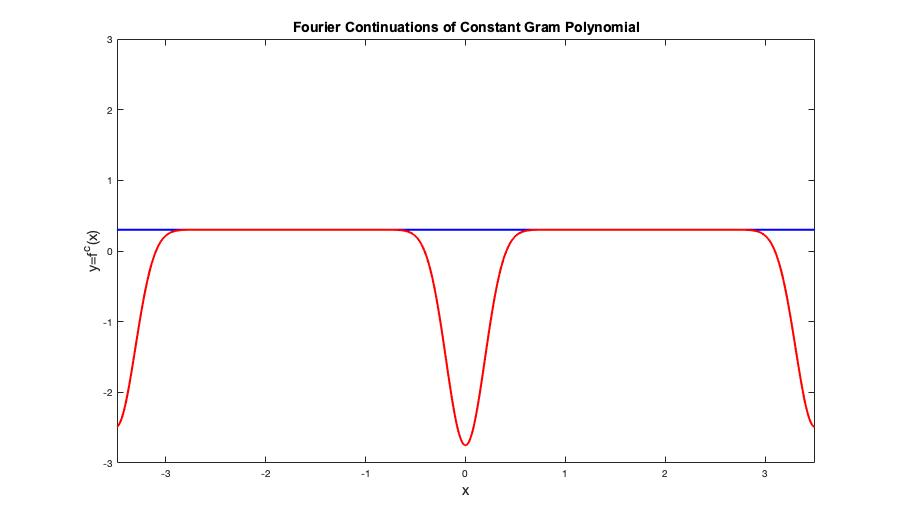
\includegraphics[scale = .4]{FourierContinuations.jpg}
\caption{Two different Fourier Continuations for a degree 0 polynomial. Both give approximately 18 digits of accuracy.}
\label{fig:Fig1}
\end{center}
\end{figure}
This means that it is possible for a procedure to ``choose" a Fourier Continuation Approximation for which energy builds in the continuation region, and then will spread back into the original domain under the inverted operator.  This can cause an unstable result.  In Figure \ref{fig:Fig1} we see that for no trade in accuracy, the blue line gives us an unstable result, while the red line gives us a stable result. \\

\subsection{What We've Done} 
We originally planned to explore the Singular Value Decomposition (SVD) of the system and try to exploit the zero singular values, but that proved to be ineffective in changing the shape of the continuation.  \\
We determined that by adding extra constraints to the system we're solving, we will be able to have more control over the system in question. Some fruitful results have come from focusing on a known solution to the BVP: The Green's Function. For simplicity, we assume that $a=-1$ and $b=b$ and that we have zero Boundary Conditions (BCs). 
\subsubsection{Green's Functions}
We calculate the Green's Function via the methods described in Bender and Orszag: Let 
\begin{equation}
G(x,a)=\begin{cases}
A_1(a)h_1(x)+B_1(a)h_2(x) & x<a \\
A_2(a)h_1(x)+B_2(a)h_2(x) & x \geq a
\end{cases}
\end{equation}
where $h_1(x)$ and $h_2(x)$ are the homogeneous solutions to  $(I-\alpha \frac{\partial^2}{\partial x^2})u=f$:

\begin{eqnarray}
h_1(x) &=& e^{\frac{(x-b)}{\sqrt{\alpha}}} \\
h_2(x) &=& e^{\frac{(-x-1)}{\sqrt{\alpha}}},
\end{eqnarray}

where $h_1$ and $h_2$ have been normalized to $1$ on the boundary.  $A_1$,$A_2$,$B_1$, and $B_2$ are computed to enforce continuity of the Green's Function, at most a small jump discontinuity of the Green's Function, and zero boundary conditions (Citation for B, O Asymptotics book).  The Green's Function for our BVP ends up being

\begin{equation}
G(x,a)=\begin{cases} 
-\dfrac{1}{2} \dfrac{\sqrt{\alpha}\left(-e^{\frac{-1-2b+a}{\sqrt{\alpha}}}+e^{-\frac{a+1}{\sqrt{\alpha}}}\right)\left(-e^{\frac{2(2+b+x)}{\sqrt{\alpha}}}+e^{\frac{2(x+1)}{\sqrt{\alpha}}}+e^{\frac{2(1+b)}{\sqrt{\alpha}}}-1\right)e^{\frac{-x+1+2b}{\sqrt{\alpha}}}}{\left(e^{\frac{2(1+b)}{\sqrt{\alpha}}}-1\right)^2} & x<a \\
\dfrac{1}{2} \dfrac{\sqrt{\alpha} \left(e^{\frac{2+b+a}{\sqrt{\alpha}}} -e^{\frac{a-b}{\sqrt{\alpha}}}\right)\left(e^{\frac{2(-x+b)}{\sqrt{\alpha}}}+e^{\frac{2(1+b)}{\sqrt{\alpha}}}-e^{\frac{2+4b-2x}{\sqrt{\alpha}}}-1\right)e^{\frac{2+b+x}{\sqrt{\alpha}}}}{\left(e^{\frac{2(1+p)}{\sqrt{\alpha}}}-1\right)^2} & x \geq a

\end{cases}
\end{equation}

To calculate the Green's Function solution to the BVP we use
\begin{equation}
u_G=\int_{-1}^b G(x,a)f(a)da.
\end{equation}
We then force the Fourier Continuation to match the function itself, and then force the inverted differential operator applied to the Fourier Continuation to match the Green's Function solution.  Since the Green's Function solution enforces zero BCs, we actually set up the equation to allow for fluctuation using the homogeneous solutions as-is, i.e. that  $(I-\alpha \frac{\partial^2}{\partial x^2})^{-1}f + a_1 h_1 + a_2 h_2 = u_G$. \\
Discretized on our grid, we use a Discrete Fourier Transform (DFT) Matrix, called $A$ to represent the Fourier Continuation operation, and $D$ to represent the differential operator.  \\
We end up making some choices about the shape of the DFT Matrix, The resulting system of equations is: 


\begin{equation}
\left[
\begin{array}{c:c}
A &  \mathbf{0} \\[6pt] \hdashline
(DA)^{\dagger} & h_1|_{\text{grid}} h_2|_{\text{grid}} \\[6pt]
\end{array} \right] 
\left[ 
\begin{array}{c}
f_c \\
a_1\\
a_2
\end{array}
\right]
= 
\left[ 
\begin{array}{c}
f|_{\text{grid}}\\
u_G|_{\text{grid}}
\end{array}
\right]
\end{equation}

\subsubsection{Enforcing Stability Via Homogeneous Solutions}
We found that the system above didn't always give us the stability we desired. To remedy this, we force a weight towards the Green's Function Solution by allowing the coefficients of that equation to be larger.  We achieve this by exploiting the fact that the SVD of the system will minimize the coefficients and adding the equation $\lambda a_1 h_1 + \lambda a_2 h_2 = 0$ to the system.  By taking $\lambda$ small, $a_1$ and $a_2$ will be larger.  By appropriately choosing $\lambda$ we are able to control the continuation and achieve stability. 
The resulting system of equations is: 
\begin{equation}
\left[
\begin{array}{c:c}
A &  \mathbf{0} \\[6pt] \hdashline
(DA)^{\dagger} & h_1|_{\text{grid}} h_2|_{\text{grid}} \\[6pt] \hdashline
\mathbf{0} & \lambda h_1|_{\text{grid}}  \lambda h_2|_{\text{grid}} \\ [6pt]
\end{array} \right] 
\left[ 
\begin{array}{c}
f_c \\
a_1\\
a_2
\end{array}
\right]
= 
\left[ 
\begin{array}{c}
f|_{\text{grid}}\\
u_G|_{\text{grid}}\\
\mathbf{0}
\end{array}
\right],
\end{equation}
where $\mathbf{0}$ represents a matrix of zeros of appropriate row and column length.  




\subsection{Using the Continuations}

\subsection{Implementation}
We chose to implement the solver in the Julia computing language.  This choice was made because Julia has a storage type \texttt{BigFloat} which allows for arbitrary precision as opposed to the double-precision (64-bit).  Setting the precision in Julia to 200 bits allows us to do calculations with an accuracy of approximately $\mathcal{O}(10^{-60})$, so even losing digits due to round-off error in solving the system, we still get a very high-accuracy result.  Using Julia packages \texttt{LinearAlgebra}, \texttt{SymPy}, \texttt{GenericSVD} and several proprietary functions, we recreated the system above and solved it using a reduced QR Factorization (Citation: Golub \& Van Loan).




\subsection{Results} 
\section{Future Work} 
\subsection{Computational Work} 
We are going to use this to put as a time step of the heat equation and solve that PDE.  Our goal is to show that we have a stable approximation that can be used. 
\subsection{Analytical Work} \\
The result that yields the same Fourier coefficients for any given Gram polynomial independent of choice of $\alpha$ is unexpected.  Our goal is to develop an analytic proof that justifies this result in general. \\




\end{document}  